% explains why yours is the best possible design
% helps others avoid dead ends
%
% your final design is typically the result of exploring a tree
%
% keep intro and walkthrough short by explaining only 
% in a separate design section mention dead ends
% do not drill deeper into dead ends though
%
\section{Design}
%
To create our device we used five techniques 
to observe the target group's needs and funnel those 
into an ever more refined design. 
\begin{description}
  \item[User Study] From the start we did not intend to win new customers to 
    the social-web idea, instead we focused on existing users
    of services like Twitter or Facebook\registered. 
    We believe that social networks are the Web 2.0 killer application. 
    Their user base is ever growing and at the same time, mobile devices
    become increasingly more popular. We feel that demand for a union of 
    those two phenomena has risen considerably, and this was supported through our preliminary 
    user study.
  \item[Contextual Inquiry]
    During a contextual inquiry we were able to identify some stereotypical 
    target users and created common task descriptions those users would 
    attempt most often. The features used by our participants differ largely, ranging 
    from ``staying in touch'' using messages to just having an ``automatic 
    birthday reminder''. Most commonly used were the messaging functionality and
    sharing photos with friends.
\begin{figure}[h]
 \begin{center}
   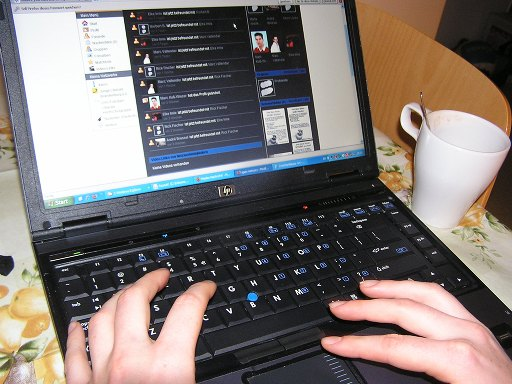
\includegraphics[width=0.8\linewidth]{imgs/context.png}
 \end{center}
 \caption{The Typical Usage Situation of a Social Network}
 \label{fig:context}
\end{figure}
  \item[Task Analysis]
    In order to further specify the tasks we want to offer with the \emph{SocioPath}
    we prepared a questionnaire for our target audience. After completing the 
    survey, we had identified a final set of tasks our users perform most often. 
    Additionally, we asked what the users perceived as the most daunting drawbacks
    of accessing their network from a browser on a computer workstation. It turned 
    out, that indeed the number of steps needed to get to a particular feature
    is seen as \emph{the} most annoying part of social networks. We considered 
    that for our design sketches and also took this as reconciliation, that our 
    goal of ubiquitous, quick access networking is indeed what users crave for.
  \item[Functionality and Design]
    Sketching as the most basic way to design user interfaces has produced 
    a great many routes for us. We have played around with different form-factors 
    and sizes, like watches, wristbands, rings or necklaces. The very small 
    size of our screen lead to some interesting input designs, we considered
    back-of-device interaction, voice input and different text input techniques
    e.g. a \emph{peep-hole} keyboard or the Palm\registered Graffiti2
    technology. The large number of sketches was then reviewed together with a 
    select group of people from our user study. We ended up prototyping a fairly 
    conservative device with a standard touchscreen and text recognition for 
    handwriting with the index finger. Due to the small screen we went for large 
    icons and few options per screen.
\begin{figure}[h]
  \begin{center}
    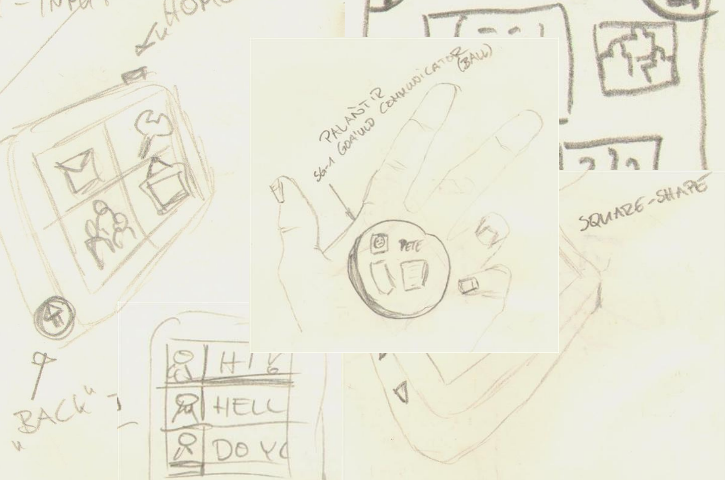
\includegraphics[width=1.0\linewidth]{imgs/sketches.png}
  \end{center}
  \caption{A Selection of Sketches for Interface Studies}
  \label{fig:sketches}
\end{figure}
  \item[Usability Flaws and Paper Prototyping]
    To further refine our design, we asked other members of the HCI course
    to evaluate what we had done to that point. We created a paper prototype
    which helped us greatly to finalize the physical design and to create 
    what we believe is a very
    discoverable device. The final device features a front-operated touch
    screen, a thumb-wheel and a ``Back'' button. The thumb-wheel here is 
    mainly a convenience, as its operations can also be done with a swipe
    gesture
    on the screen, however, some of our testers exclaimed they were more
    comfortable with a wheel, both for the physical sensation as well 
    as for operating the device eyes-free.

    To discover UI usability flaws in a heuristic evaluation we 
    created a link map
    of all our screens. At that time the device design was already 
    reasonably finalized so that we could focus on the software side of
    things. While our ideas were deemed pretty accessible as they were, 
    a few cosmetic flaws were pointed out, which we duly incorporated into
    our link map, e.g. our reliance on iconic representation was criticized
    for leaving to much space for interpretation. To resolve this issue, 
    we added an action name that appears when an icon is in focus, to 
    reassure the user.
  \item[Interactive Prototype]
    The interactive prototype represents our finalized UI design. Although
    we did not implement the final graphics, the prototype gives a very 
    thorough impression of the ``feel'' we intend for the software to have.
    All screens from our link map, enhanced with the experiences gathered 
    from our evaluation, are present in the prototype and their behavior 
    was simulated as best as possible using mouse and keyboard.

    The final UI favors horizontal and vertical scrolling as well as item
    expansion over switching between lots of screens. The main menu has 
    large icons for quick access and a ticker with notifications at the top.
    Input is always full screen and a faint ``Just write'' written on the
    background hints at how text input is intended. If the user hesitates,
    the device assumes he still does not know what to do, and a short 
    animation of a finger writing on the screen appears.\\ 
    The detail pages of friends and the message board is a vertically 
    scrolling list of items, each of which only displays a maximum of 
    two rows of text. Tapping an item expands it and the user can read 
    more by simply scrolling down further.

    In a list, we use a glowing line on top and bottom to indicate more 
    items in either direction, if there are any. We use this technique 
    because we cannot always assure that the next item to the top or 
    bottom is ``cut-of'' to indicate more content, as expanded items can
    be of arbitrary length.
\begin{figure}[h]
  \begin{center}
    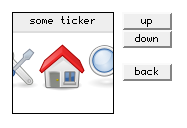
\includegraphics[width=0.6\linewidth]{imgs/screen.png}
  \end{center}
  \caption{A Screenshot of the Interactive Prototype}
  \label{fig:prototype}
\end{figure}
\end{description}
